\documentclass{article}
\usepackage[utf8]{inputenc}
\usepackage{amsmath}
\usepackage{amssymb}
\usepackage{graphicx}

\newcommand\xkn{\mathbf{x}^{\left(k+1\right)}}
\newcommand\xk{\mathbf{x}^{\left(k\right)}}
\newcommand\A{\mathbf{A}}
\newcommand\DA{\mathbf{D}_{\mathbf{A}}}
\newcommand\LA{\mathbf{L}_{\mathbf{A}}}
\newcommand\UA{\mathbf{U}_{\mathbf{A}}}
\newcommand\xstar{\mathbf{x}^{*}}

\begin{document}

\section*{Symmetric Gauss-Seidel iteration}
We define for a square matrix $\mathbf{A}\in \mathbb{R}^{n,n}$ matrices $\mathbf{D}_{A}, \mathbf{L}_{A}, \mathbf{U}_{A} \in \mathbb{R}^{n,n}$ by
\begin{equation*}
    \left(\mathbf{D}_{\mathbf{A}}\right)_{i,j} := \begin{cases}
    \left(\mathbf{A}\right)_{i,j}\,,\: &i = j\,, \\
    0\,, &i\neq j
    \end{cases}, \left(\mathbf{L}_{\mathbf{A}}\right)_{i,j} = \begin{cases} 
    \left(\mathbf{A}\right)_{i,j} \,,\: &i > j \,, \\
    0\,, & i\leq j
    \end{cases}\, \left(\mathbf{U}_{\mathbf{A}}\right)_{i,j} := \begin{cases}
        \left(\mathbf{A}\right)_{i,j}\,,\: &i < j \\
        0 \,, &i \geq j
    \end{cases}
\end{equation*}
We hence have for 
\begin{equation*}
    \mathbf{A} = \begin{bmatrix}
    a_{11} & a_{12} & \dots & a_{1n} \\
    a_{12} & a_{22} & \dots & a_{2n} \\
    \vdots & \vdots &  \ddots& \vdots \\
    a_{n1} & a_{n2} & \dots & a_{nn}
    \end{bmatrix}
\end{equation*}
for the matrix $\mathbf{D}_{\mathbf{A}}$
\begin{equation*}
\mathbf{D}_{\mathbf{A}} = 
    \begin{bmatrix}
        a_{11} & 0 & \dots & 0 \\
    0 & a_{22} & \dots & 0 \\
    \vdots & \vdots & \ddots & \vdots \\
   0& 0 & \dots & a_{nn}
    \end{bmatrix}
\end{equation*}
for the matrix $\mathbf{L}_{\mathbf{A}}$
\begin{equation*}
\mathbf{L}_{\mathbf{A}} =
    \begin{bmatrix}
        0 & \dots & 0 & 0 \\
    a_{12} & \dots & 0 & 0 \\
     \vdots & \ddots & \vdots & \vdots \\
    a_{n1} & \dots & a_{nn-1} &0
    \end{bmatrix}
\end{equation*}
and for the matrix $\UA$
\begin{equation*}
\UA = 
    \begin{bmatrix}
    0 & a_{12} & \dots & a_{1n} \\
    0 & 0 & \ddots & \vdots \\
    \vdots & \vdots &  \ddots& a_{n-1\,n} \\
    0 & 0 & \dots & 0
    \end{bmatrix}
\end{equation*}
The symmetric Gauss-Seidel iteration associated with the linear system of equations $\mathbf{A}\mathbf{x} = \mathbf{b}$ is defined as 
\begin{equation*}
    \xkn = \left(\UA + \DA\right)^{-1}\mathbf{b} - \left(\UA + \DA\right)^{-1}\LA\left(\LA + \DA\right)^{-1}\left(\mathbf{b}- \UA \xk\right)
\end{equation*}
\subsection*{1-12.a}
We are tasked with giving a necessary and sufficient condition on $\mathbf{A}$, such that the symmetric Gauss-Seidel iteration above is well-defined. For the symmetric Gauss-Seidel iteration to be well-defined all matrices that are inverted must be invertable, i.e. regular. Let us look at the matrices in question, first we have $\UA + \DA$
\begin{equation*}
    \UA + \DA = 
    \begin{bmatrix}
    0 & a_{12} & \dots & a_{1n} \\
    0 & 0 & \ddots & \vdots \\
    \vdots & \vdots &  \ddots& a_{n-1\,n} \\
    0 & 0 & \dots & 0
    \end{bmatrix}+\begin{bmatrix}
        a_{11} & 0 & \dots & 0 \\
    0 & a_{22} & \dots & 0 \\
    \vdots & \vdots & \ddots & \vdots \\
   0& 0 & \dots & a_{nn}
    \end{bmatrix} = \begin{bmatrix}
    a_{11} & a_{12} & \dots & a_{1n} \\
    0 & a_{22} & \dots & a_{2n} \\
    \vdots & \ddots &  \ddots& \vdots \\
   0 & \dots & 0 & a_{nn}
    \end{bmatrix}
\end{equation*}
The matrix $\UA + \DA$ is hence the upper triangular part of $\mathbf{A}$ and as such is regular if and only if the product of all its diagonal elements is non-zero (as then the determinant is non-zero for a triangular matrix). The product of its diagonal elements is given by
\begin{equation*}
    \prod_{i=0}^{n} a_{ii} \neq 0 \Longleftrightarrow a_{ii} \neq 0 \quad \forall \, i \in \left\{1, \dots, n\right\}
\end{equation*}
the other matrix that must be invertible is given by $\LA + \DA$ which looks like
\begin{equation*}
    \LA + \DA = \begin{bmatrix}
        0 & \dots & 0 & 0 \\
    a_{12} & \dots & 0 & 0 \\
     \vdots & \ddots & \vdots & \vdots \\
    a_{n1} & \dots & a_{nn-1} &0
    \end{bmatrix} + \begin{bmatrix}
        a_{11} & 0 & \dots & 0 \\
    0 & a_{22} & \dots & 0 \\
    \vdots & \vdots & \ddots & \vdots \\
   0& 0 & \dots & a_{nn}
    \end{bmatrix} = \begin{bmatrix}
    a_{11} & 0 & \dots & 0 \\
    a_{12} & a_{22} & \ddots & \vdots \\
    \vdots & \vdots &  \ddots& 0 \\
    a_{n1} & a_{n2} & \dots & a_{nn}
    \end{bmatrix}
\end{equation*}
which is the lower triangular part of $\mathbf{A}$, the same exact condition applies here for it to be regular. Hence we can conclude that the necessary (otherwise the iteration is not well-defined) and sufficient (with it the iteration is well-defined) is given by
\begin{equation*}
    a_{ii} \neq 0 \quad \forall \, i \in \left\{1, \dots, n\right\}
\end{equation*}
\subsection*{1-12.b}
Assuming that the symmetric Gauss-Seidel iteration is well-defined, we are tasked to show that a fixed point $\mathbf{x}$ of the iteration is a solution of the linear system of equations $\mathbf{A}\mathbf{x} = \mathbf{b}$. Let hence $\mathbf{x}$ be a solution to the LSE $\mathbf{A}\mathbf{x} = \mathbf{b}$. Let us define for easier notation the "next-step" function $\Phi\left(\mathbf{x}\right)$ by
\begin{equation*}
    \Phi\left(\mathbf{x}\right) = \left(\UA + \DA\right)^{-1}\mathbf{b} - \left(\UA + \DA\right)^{-1}\LA\left(\LA + \DA\right)^{-1}\left(\mathbf{b}- \UA \mathbf{x}\right)
\end{equation*}
the point $\mathbf{x}$ would be a fixed-point to the iteration if we get $\Phi\left(\mathbf{x}\right) = \mathbf{x}$. Let us take a closer look at the three matrices $\UA$, $\LA$ and $\DA$, we have
\begin{equation*}
    \mathbf{A} = \LA + \DA + \UA
\end{equation*}
hence we can write the LSE $\mathbf{A}\mathbf{x} = \mathbf{b}$ as 
\begin{equation*}
    \mathbf{A}\mathbf{x} = \mathbf{b} \Longleftrightarrow \left(\LA + \DA + \UA\right)\mathbf{x} = \mathbf{b}
\end{equation*}
we hence want to reach the form on the right. Let us now try to take apart the symmetric Gauss-Seidel iteration to reach the desired form starting from $\Phi\left(\mathbf{x}\right) = \mathbf{x}$ 
\begin{align*}
   &\phantom{\Longleftrightarrow} \left(\UA + \DA\right)^{-1}\mathbf{b} - \left(\UA + \DA\right)^{-1}\LA\left(\LA + \DA\right)^{-1}\left(\mathbf{b}- \UA \mathbf{x}\right) = \mathbf{x} \\
    &\Longleftrightarrow 
    \left(\UA + \DA\right)^{-1}\left(\mathbf{b} - \LA\left(\LA + \DA\right)^{-1}\left(\mathbf{b}- \UA \mathbf{x}\right)\right) = \mathbf{x} \\
    &\Longleftrightarrow
    \mathbf{b} - \LA\left(\LA + \DA\right)^{-1}\left(\mathbf{b}- \UA \mathbf{x}\right) = \left(\UA + \DA\right)\mathbf{x} \quad \text{\big[$\left(\UA + \DA\right)^{-1}$ is invertible\big]}
\end{align*}
We define now 
\begin{equation*}
    \mathbf{y} := \left(\LA + \DA\right)^{-1}\left(\mathbf{b}- \UA \mathbf{x}\right)
\end{equation*}
this gives us
\begin{equation}
    \mathbf{b} - \LA\mathbf{y} = \left(\UA + \DA\right)\mathbf{x}
\end{equation}
 we have 
\begin{equation*}
    \mathbf{A} = \UA + \DA + \LA \Longleftrightarrow \mathbf{A} - \LA = \UA + \DA
\end{equation*}
the equation for $\mathbf{y}$ itself gives us
\begin{equation*}
    \mathbf{y} = \left(\LA + \DA\right)^{-1}\left(\mathbf{b}- \UA \mathbf{x}\right) \Longleftrightarrow  \left(\LA + \DA\right)\mathbf{y} = \mathbf{b}- \UA \mathbf{x} 
\end{equation*}
which yields
\begin{equation}
    \mathbf{b}- \UA \mathbf{x} = \left(\LA + \DA\right)\mathbf{y}
\end{equation}
We get the following system of equations
\begin{align*}
     \mathbf{b} - \LA\mathbf{y} &= \left(\UA + \DA\right)\mathbf{x} \\
     \mathbf{b}- \UA \mathbf{x} &= \left(\LA + \DA\right)\mathbf{y}
\end{align*}
which then yields
\begin{align*}
    \left(\UA + \DA\right)\mathbf{x} + \LA\mathbf{y} = \mathbf{b} \\
    \left(\LA + \DA\right)\mathbf{y} + \UA\mathbf{x} = \mathbf{b}
\end{align*}
we can subtract the first from the second to give us
\begin{align*}
     \left(\UA + \DA\right)\mathbf{x} + \LA\mathbf{y} -\left(\LA + \DA\right)\mathbf{y} - \UA\mathbf{x} =0 \\
     \UA\mathbf{x} + \DA\mathbf{x} + \LA\mathbf{y} - \LA\mathbf{y} - \DA \mathbf{y} - \UA\mathbf{x} = 0 \\
     \underbrace{\UA \mathbf{x} - \UA \mathbf{x}}_{=0} + \underbrace{\LA\mathbf{y} - \LA\mathbf{y}}_{=0} + \DA\mathbf{x} - \DA\mathbf{y} = 0 \\
     \DA\mathbf{x} - \DA\mathbf{y} = 0 
\end{align*}
We hence get 
\begin{equation*}
    \DA\mathbf{x} = \DA\mathbf{y}
\end{equation*}
we have shown that $\DA$ is invertible hence we have
\begin{equation*}
    \DA\mathbf{x} = \DA\mathbf{y} \implies \mathbf{x} = \mathbf{y}
\end{equation*}
Plugging this into equation (1) gives us
\begin{equation*}
    \mathbf{b} - \LA\mathbf{x} = \left(\UA + \DA\right)\mathbf{x} \implies \mathbf{b} = \left(\LA + \DA + \UA\right)\mathbf{x}
\end{equation*}
this is exactly what we wanted and hence we can conclude the proof.

\subsection*{1-12.c}
We are tasked with implementing the function \verb|GSIt| solving the linear system $\mathbf{A}\mathbf{x} = \mathbf{b}$ using the iterative scheme given by the symmetric Gauss-Seidel iteration. We are given an initial guess $\mathbf{x}^{\left(0\right)}$ passed in \verb|x| as well as the matrix $\mathbf{A}$ (passed in \verb|A|) and the right-hand side vector $\mathbf{b}$ (passed in \verb|b|). We are told to use a correction based termination criterion with a relative tolerance based on the Euclidean vector norm. The correction based criterion is defined by

\begin{figure}[!hbt]
    \centering
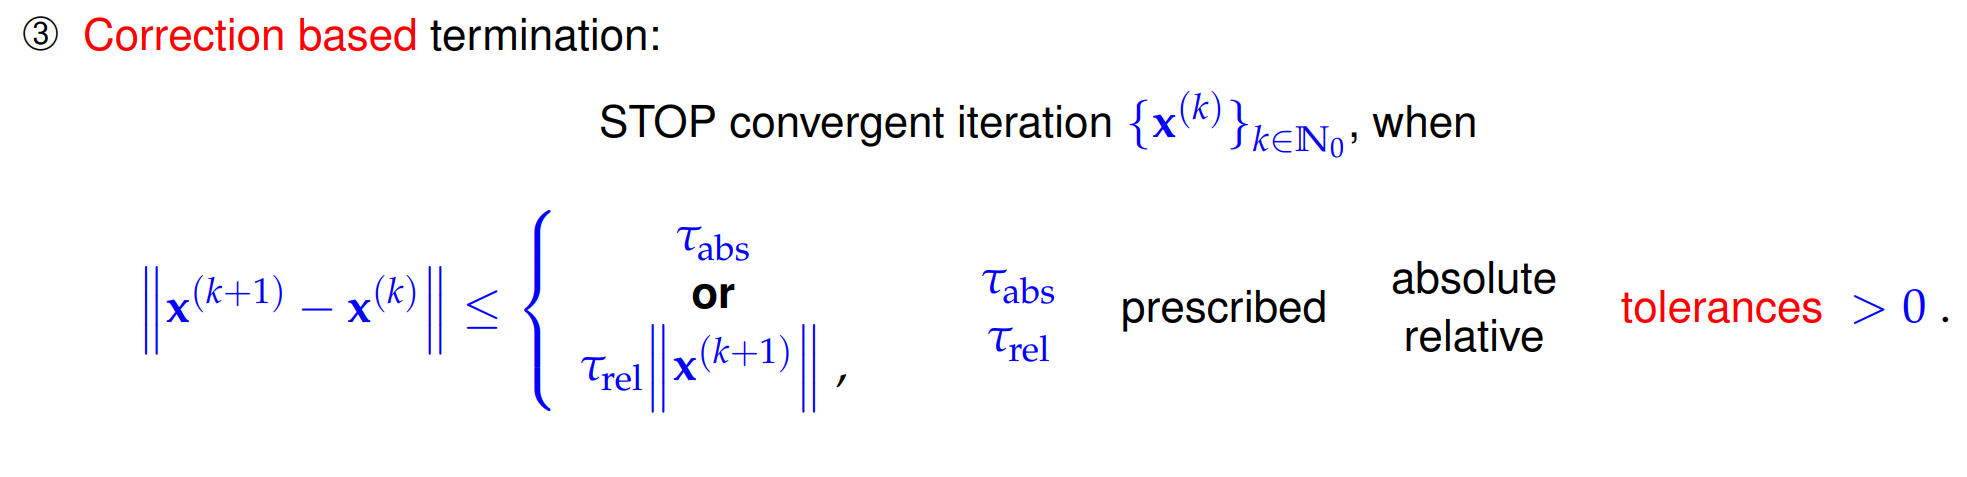
\includegraphics[width=1.0\linewidth]{CorrectionBasedCriterion.png}
\end{figure}

\noindent We will use a default tolerance of $\text{tol} = 1\cdot 10^{-8}$. The main difficulty now lies with computing the inverses of $\left(\UA + \DA\right)$ and $\left(\LA + \DA\right)$, however as we have seen the first is an upper triangular matrix and the second is a lower triangular matrix and Eigen allows us to solve systems of the form 
\begin{equation*}
    \mathbf{A}\mathbf{x} = \mathbf{y}
\end{equation*}
directly if $\mathbf{A}$ is triangular. We hence compute the following terms using this method where $\mathbf{z}$ is just some placeholder variable and has no meaning in this context.
\begin{equation*}
    \left(\UA + \DA\right)^{-1}\mathbf{b} = \mathbf{z} \Longleftrightarrow \left(\UA + \DA\right)\mathbf{z} = \mathbf{b}
\end{equation*}
we can compute $\mathbf{z}$ using \\[2mm]
\verb|(U + D).solve(b)| \\[1mm]
the next term is given by ($\mathbf{v}$ is the rest of the expression)
\begin{equation*}
    \left(\UA + \DA\right)^{-1}\LA\mathbf{v} = \mathbf{z} \Longleftrightarrow \left(\UA + \DA\right)\mathbf{z} = \LA\mathbf{v}
\end{equation*}
which we can compute using
\\[2mm]
\verb|(U + D).solve(Lv)| \\[1mm]
the last term is given by
\begin{equation*}
    \left(\LA + \DA\right)^{-1}\left(\mathbf{b} - \UA\mathbf{x}\right) = \mathbf{z} \Longleftrightarrow  \left(\LA + \DA\right)\mathbf{z} = \mathbf{b} - \UA\mathbf{x}
\end{equation*}
which we can compute using \\[2mm]
\verb|(L + D).solve(b - U * x)| \\[1mm]
We will use \verb|TriangularView| objects to store the sums of matrices and on which we can directly apply \verb|solve| on, as the sums themselves do not directly support this utility and the above is more meant as pseudocode to help understanding what we do. \\[2mm]
\verb|TriangularView<const Eigen::MatrixXd, Eigen::Upper>| \\[1mm]
The above gives us a \verb|TriangularView| object of an upper triangular matrix. We now must be aware of a little things Eigen tends to do which is \textbf{lazy evaluation}. Lazy evaluation happens when results of operations are not stored in objects of the usual type one would expect, e.g \verb|Eigen::MatrixXd|, but in some temporary storage container, this results in us not being able to apply method calls on them as they are not compatible. For example  \\[2mm]
\verb|(U + D).triangularView<Eigen::Upper>()| \\[1mm]
will fail to compile due to lazy evaluation. What we do here is force Eigen to actually evaluate the expression using the method \verb|eval()|, the following line does compile \\[2mm]
\verb|(U + D).eval().triangularView<Eigen::Upper>()| \\[1mm]
However doing this is a bad idea, as we would first have to create the matrices \verb|U|, \verb|D| and \verb|L| using various views of matrices, where we could just use \\[2mm]
\verb|U + D = A.triangularView<Eigen::Upper>()| \\
\verb|L + D = A.triangularView<Eigen::Lower>()| \\[1mm]
This gives us the following code
\begin{figure}[!hbt]
    \centering
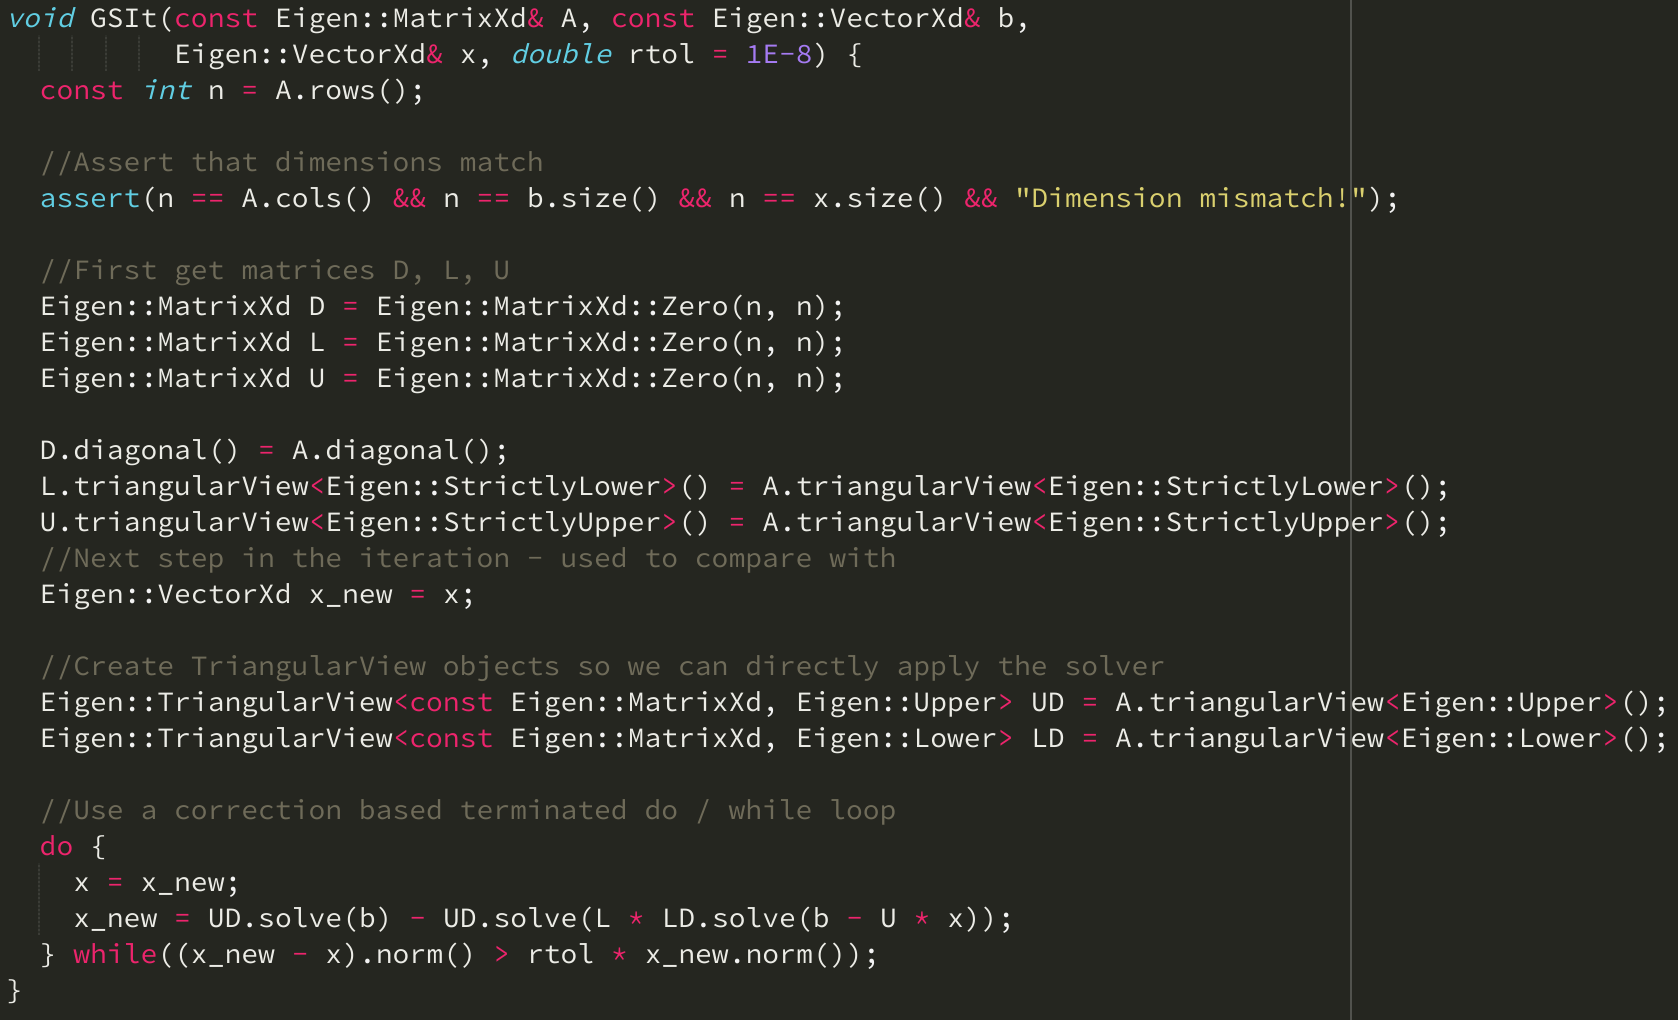
\includegraphics[width=1.0\linewidth]{1-12.c.png}
\end{figure}

\noindent It produces the same results as the master solution (which both are not always correct). I have yet to figure out why that is. As an example
\begin{equation*}
    \mathbf{A} = \begin{bmatrix}
        1 & 1 & 2 \\
        2 & 1 & 1 \\
        1 & 2 & -1
    \end{bmatrix} \quad 
    \mathbf{b} = \begin{bmatrix}
        1 \\ 2 \\ 3
    \end{bmatrix} \quad \mathbf{x}_{0} = \begin{bmatrix}
        0.8 \\
        1.0 \\
        1.5
    \end{bmatrix}
\end{equation*}
produces the same result for both methods which are both equally wrong. 

\subsection*{1-12.d}
We are now tasked with testing our implementation for $n = 9$ and $\text{rtol} = 10 \cdot 10^{-8}$ with the linear system given by
\begin{equation*}
    \mathbf{A} = \begin{bmatrix}
        3 & 1 & 0 & \dots & 0 \\
        2 & \ddots & \ddots & \ddots & \vdots \\
        0 & \ddots & \ddots & \ddots & 0 \\
        \vdots & \ddots & \ddots & \ddots & 1 \\
        0 & \dots & 0 & 2 & 3
    \end{bmatrix} \in \mathbb{R}^{n,n}\,,\quad \mathbf{b} = \begin{bmatrix}
        1 \\
        \vdots \\
        1
    \end{bmatrix} \in \mathbb{R}^{n}
\end{equation*}
we are told to output the $l^{2}$ (just the usual euclidean norm) of the \textbf{residual} $\mathbf{b} - \mathbf{A}\tilde{\mathbf{x}}$ of the approximated solution $\mathbf{x}$ and we should use $\mathbf{b}$ as the starting vector. This gives the following code.

\begin{figure}[!hbt]
    \centering
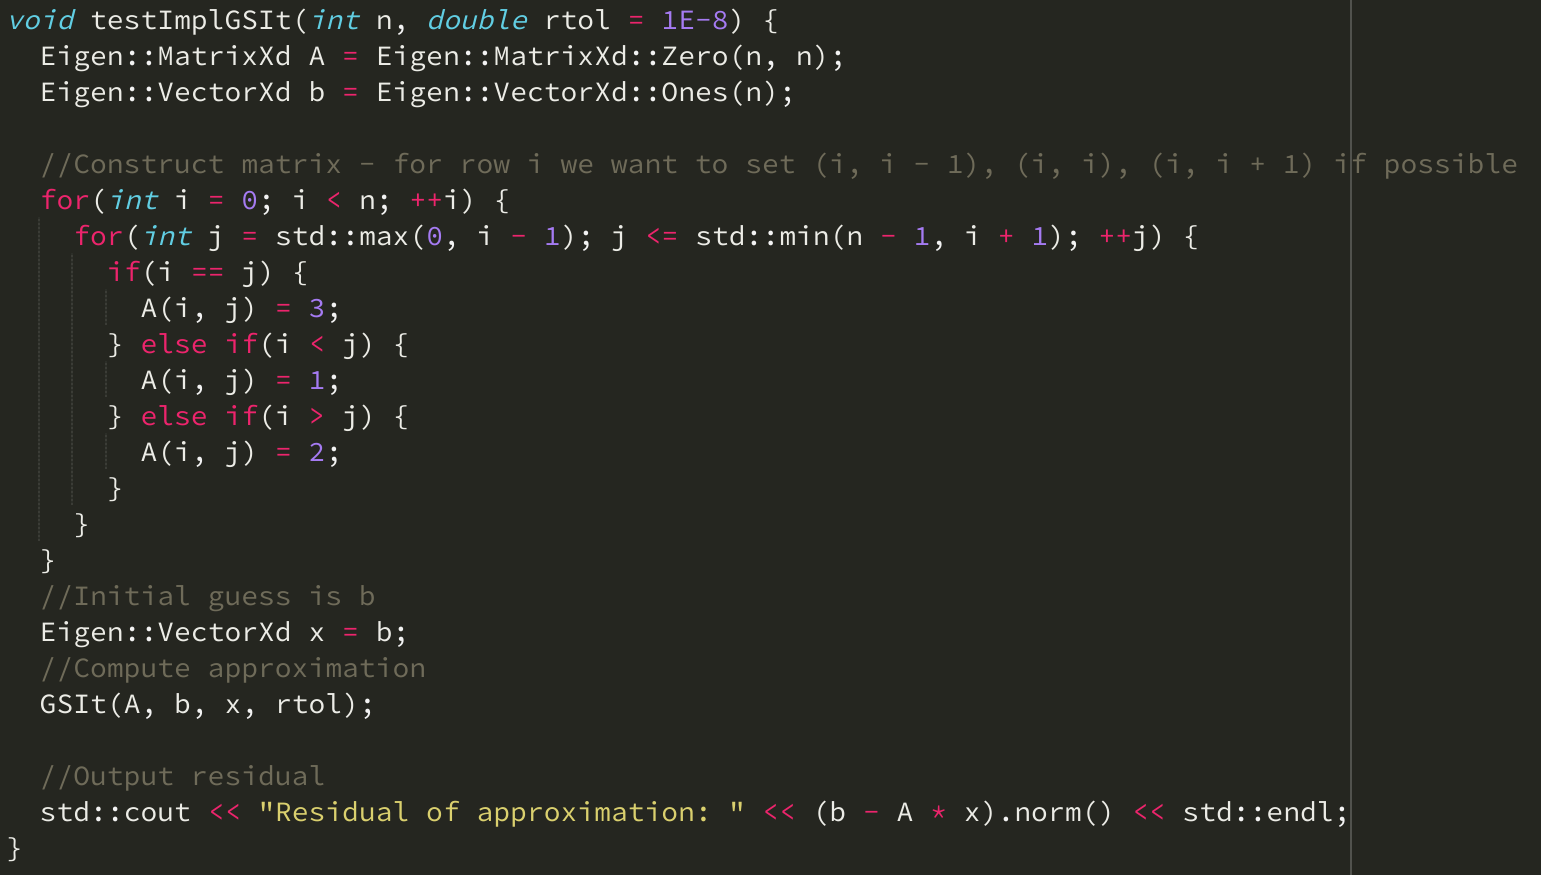
\includegraphics[width=1.0\linewidth]{1-12.d.png}
\end{figure}
\pagebreak 

\subsection*{1-12.e}
We are given the following quantities.
\begin{figure}[!hbt]
    \centering
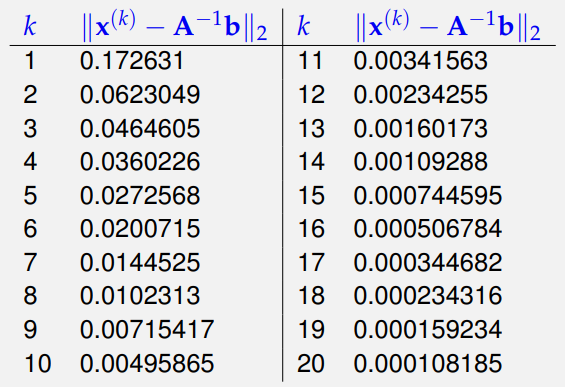
\includegraphics[width=0.5\linewidth]{1.12.e.png}
\end{figure}

\noindent and are tasked to describe the convergence rate of the iterative scheme. We look at steps $1$, $2$, $4$, $8$ and $16$ and see that the approximation error norm between $\xk$ and the exact result $\mathbf{A}^{-1}\mathbf{b}$ is halfed every time the iteration steps double, hence we can say that we can expect linear convergence.

\end{document}
